\documentclass[Rapport/Rapport_main.tex]{subfiles}

\begin{document}

\subsection{Cup Sensor}
Lyset for hvert CupLight skal i UC1 og UC2 styres på baggrund af om der er placeret en kop, og i UC2 om en bold er ramt i en kop. Derudover skal RPi vide hvilke kopper der er placeret på en given playerside da den skal vide hvornår spillet er færdigt.
\subsubsection{Hardware Design}
For at detektere placering af kop, og at bold rammer i en kop, er der udført en teknologiundersøgelse (afsnit \fullref{hwdesign:sec:CupSensorTekUnder} i Hardwaredesign bilaget). I denne undersøgelse, overvejes forskellige egenskaber en kop med øl har, som kan måles. Det overvejes bl.a. at koppen har en masse, koppen påvirker lys, og koppen har en anden dielektricitetskonstant end luft. Der undersøges i detalje sensorer der måler de to sidste egenskaber, en kapacitiv sensor og en optisk sensor. Disse to sensorer sammenlignes og bl.a. fordi den optiske sensor viste bedste tegn til at detektere at en bold rammer i, vælges denne metode, på trods at et lavere signal-støjforhold.

\begin{figure}[H]
    \centering
    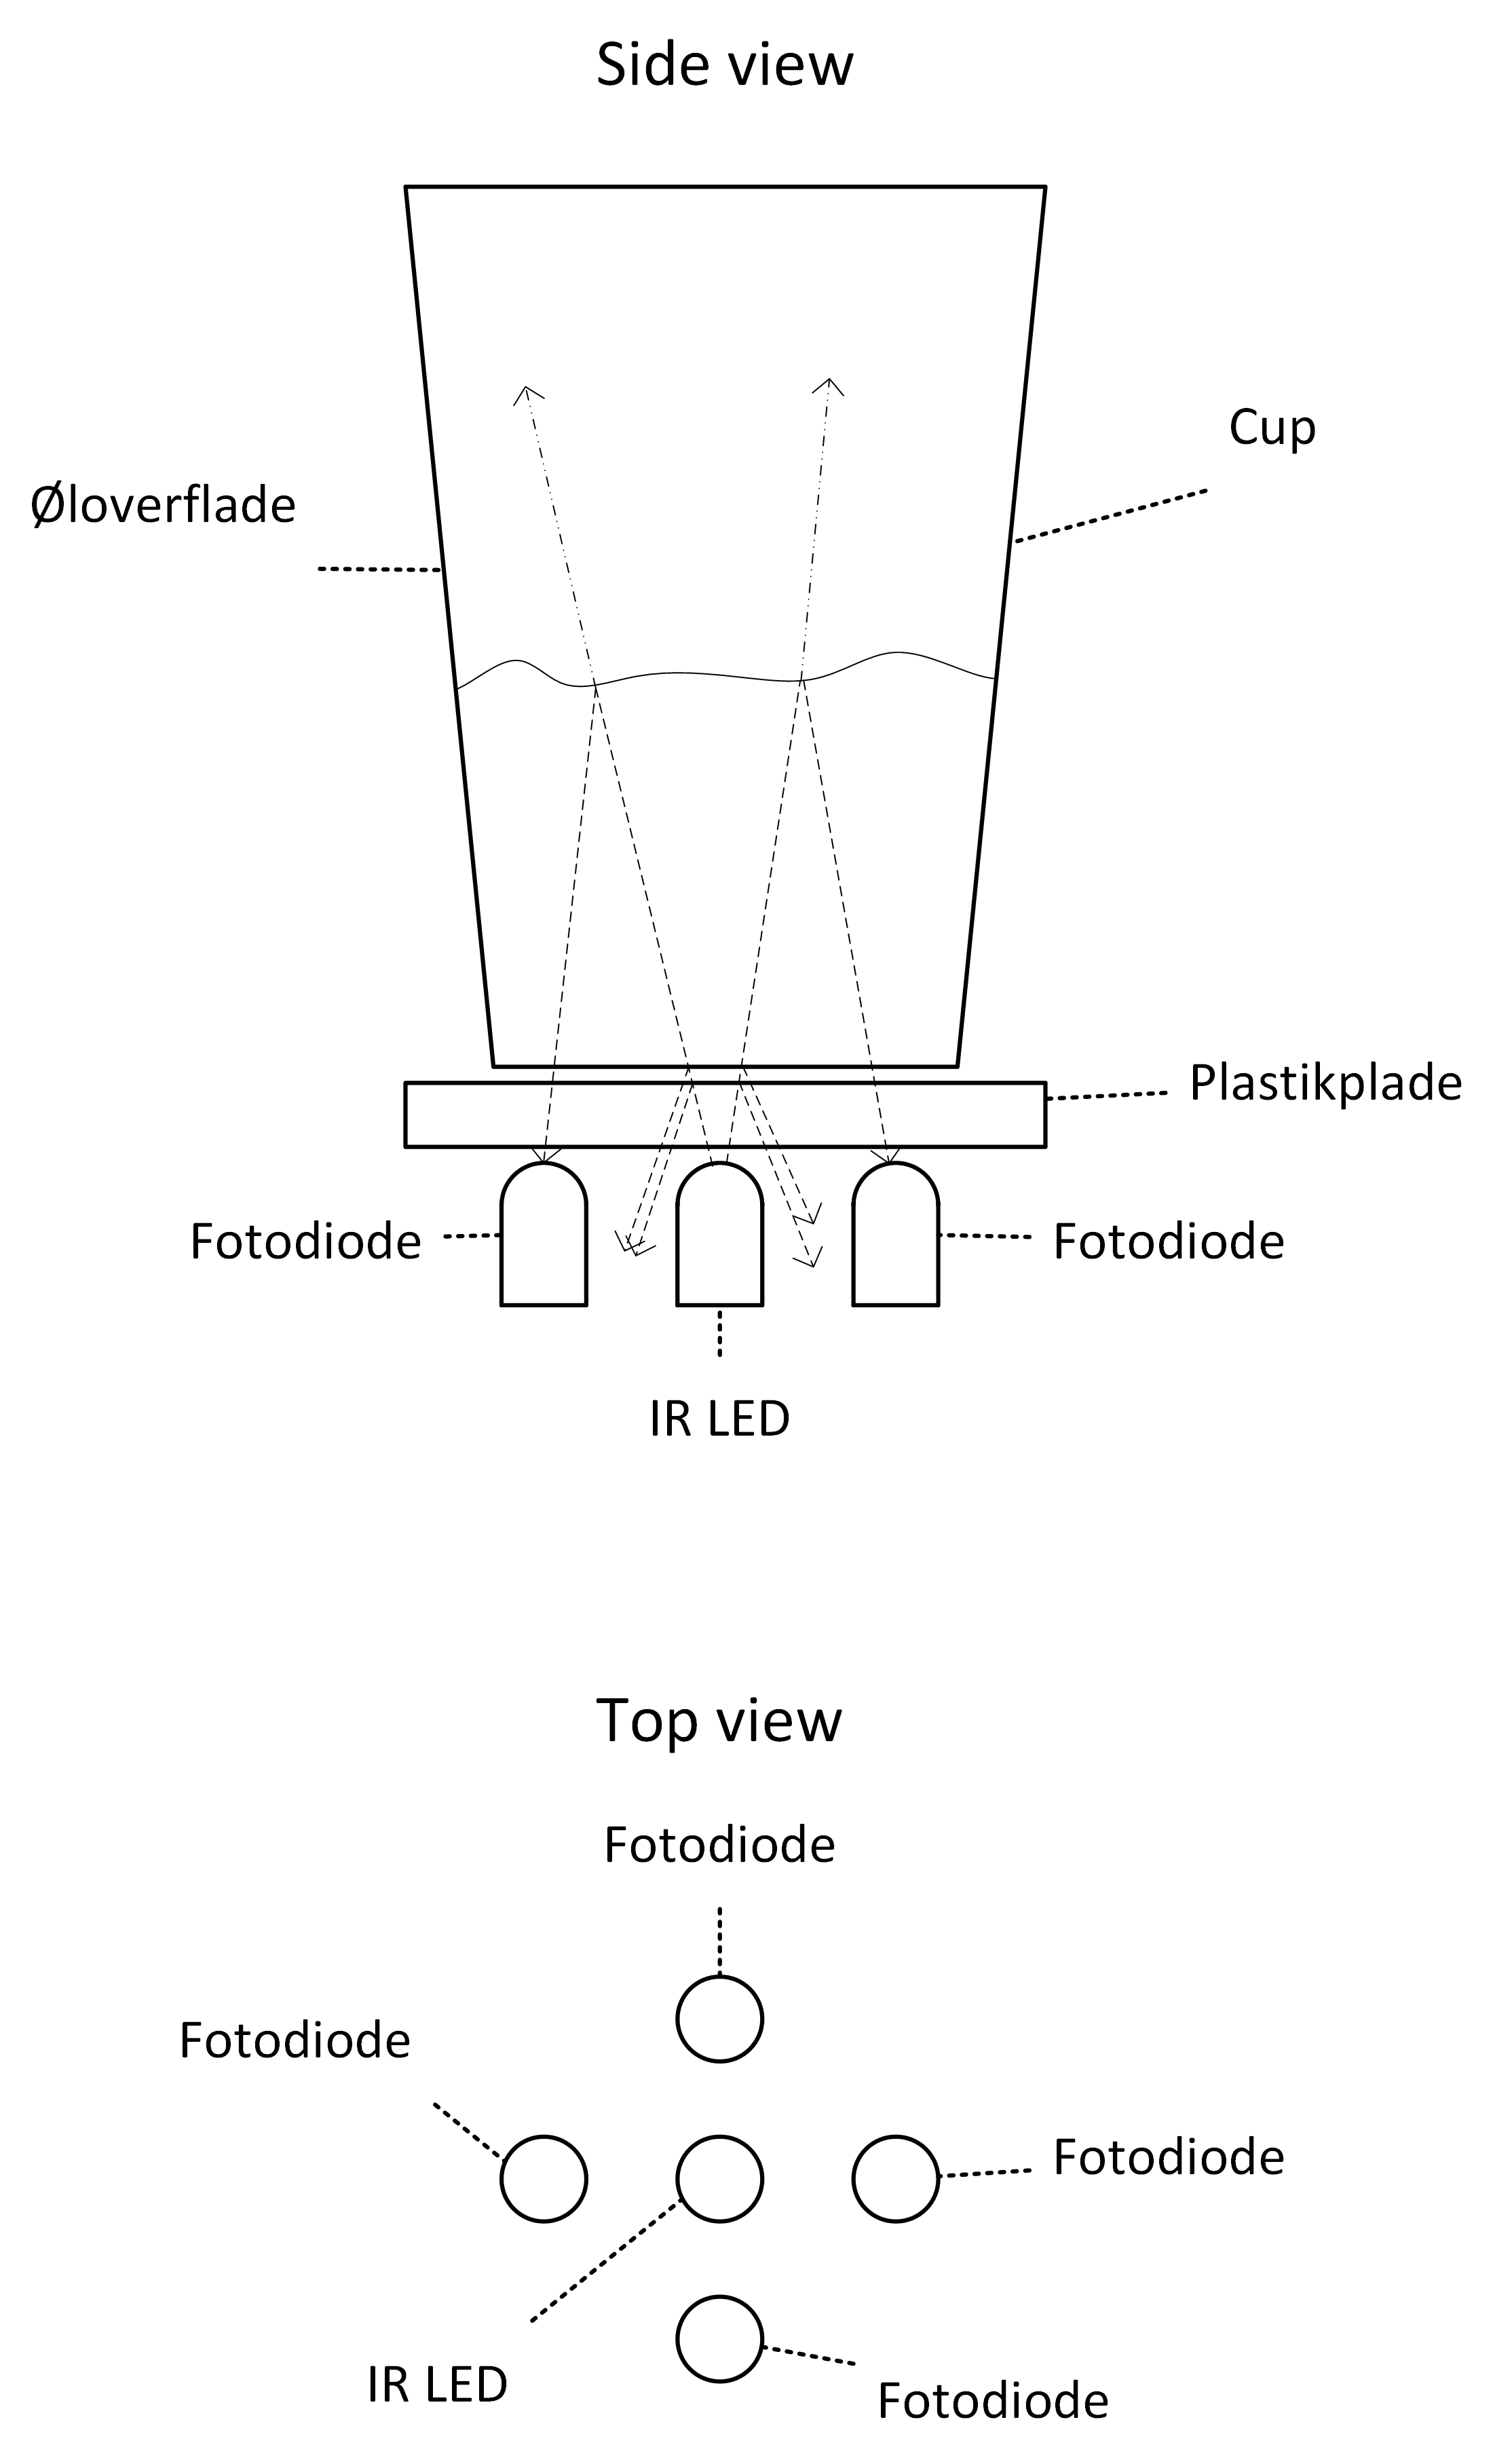
\includegraphics[width=0.8\textwidth]{HardwareDesign/CupSensor/graphics/lightPath.png}
    \caption{Her ses hvordan opstillingen af sensoren skal være. Både fra siden og fra toppen. Der benyttes én IR LED, og fire fotodioder. Der er derudover tegnet Cup med øl og gennemsigtig plastikplade på skitsen. Der er også påtegnet hvordan det tænkes lyset vil bevæge sig}
    \label{fig:lightPaht}
\end{figure}

For at lave en optiske sensor benyttes der opstillingen som ses på \ref{fig:lightPaht}. Der benyttes en IR LED som lyser op i centrum af koppen og 4 fotodioder som er sensitive over for det lys som LED'en udsender. Der blev i teknologiundersøgelsen kun brugt 2 fotodioder på hver side af LED'en, men det blev observeret at signalet fra sensoren varierede meget afhængig af hvor bolden er i koppen. Derfor blev der benyttet 4, som placeres i en ring rundt om LED'en. Det blev i teknologiundersøgelsen også bestemt at den optimale afstand mellem LED og en fotodiode er ca. 10mm. Kredsløbet kan ses på figur \ref{fig:CupSensorDesign}  
\begin{figure}[H]
    \centering
    \makebox[\textwidth][c]{%
        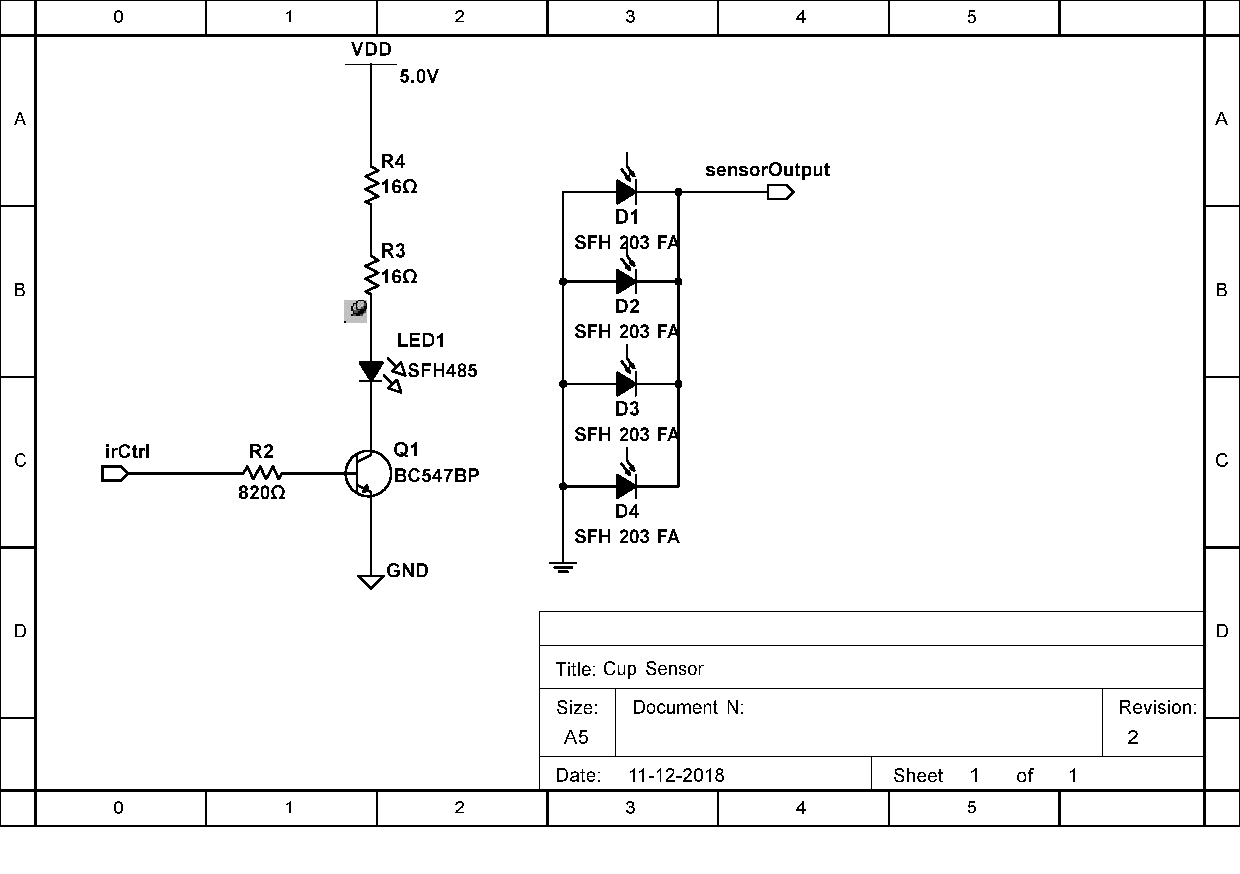
\includegraphics[width=1\columnwidth,trim={0.6in 1.8in 2.6in 0.25in},clip, page=1]{HardwareDesign/CupSensor/graphics/FinalDesign/CupSensor.pdf}
    }
    \caption{Design af Cup Sensor.}
    \label{fig:CupSensorDesign}
\end{figure}
Fotodioder virker på den måde at der i spæreretningen løber en strøm afhængig af lysintensiteten. Omgivelserne kan variere meget, og der kommer et DC offset, hvis systemet fx. bruges udendørs i sollys. Derfor er det valgt at blinke med LED'en, som styres vha. 'irCtrl', og nyttesignalet er derfor et AC signal. Til at sortere DC'en væk, bruges kredsløbet som ses på figur \ref{fig:CupSensorCupHolderControllerPart}, som fungerer som et højpas filter. Her forbindes 'sensorOutput' fra figur \ref{fig:CupSensorDesign} fra alle 6 Cup Sensor's til 'sensors' på figur \ref{fig:CupSensorCupHolderControllerPart}, som er en del af Cup Holder Controller. 
\begin{figure}[H]
    \centering
    \makebox[\textwidth][c]{%
        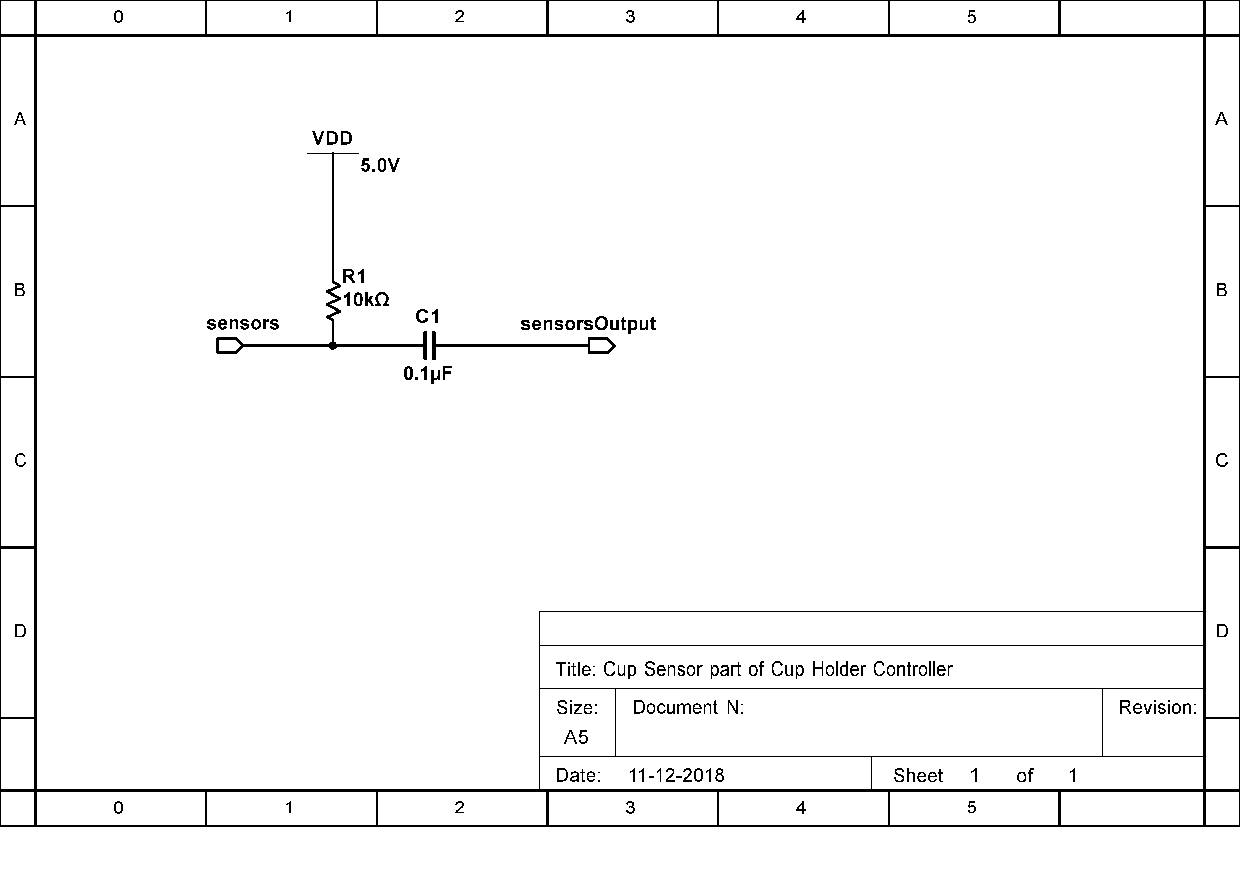
\includegraphics[width=0.7\columnwidth,trim={1.3in 3in 3.8in 0.5in},clip, page=1]{HardwareDesign/CupSensor/graphics/FinalDesign/CupSensorPart-CupHolderController.pdf}
    }
    \caption{Den del af Cup Holder Controller som sørger for at modtage signalet fra alle sensorer og filtrere DC fra.}
    \label{fig:CupSensorCupHolderControllerPart}
\end{figure}

Derudover benyttes der på PSoC'en en TIA til at konvertere strømsignalet til en spænding. Vha. mixerfunktionallitet indbygget i en Delta Sigma ADC laves der et båndpasfilter. På denne måde er DC niveauet fra ADC'en kun afhængig af det lys der sendes fra den infrarøde LED, da DC signaler og fx. 50Hz lys sorteres fra.

PSoC Komponenten kan ses på figur \ref{fig:CupSensorPSoCDesign}. Det ses at der bruges en demultiplexer, hvor hvert output ledControl0, ledControl1 ..., styrer LED'erne på hver Cup Sensor. På denne måde kan det vha. Control\_Red\_Led styres hvilken Cup Sensor's LED der skal blinke og dermed modtages der kun signalet fra denne sensor, selvom alle fotodioderne er forbundet til hinanden.  

\begin{figure}[H]
    \centering
    \makebox[\textwidth][c]{%
        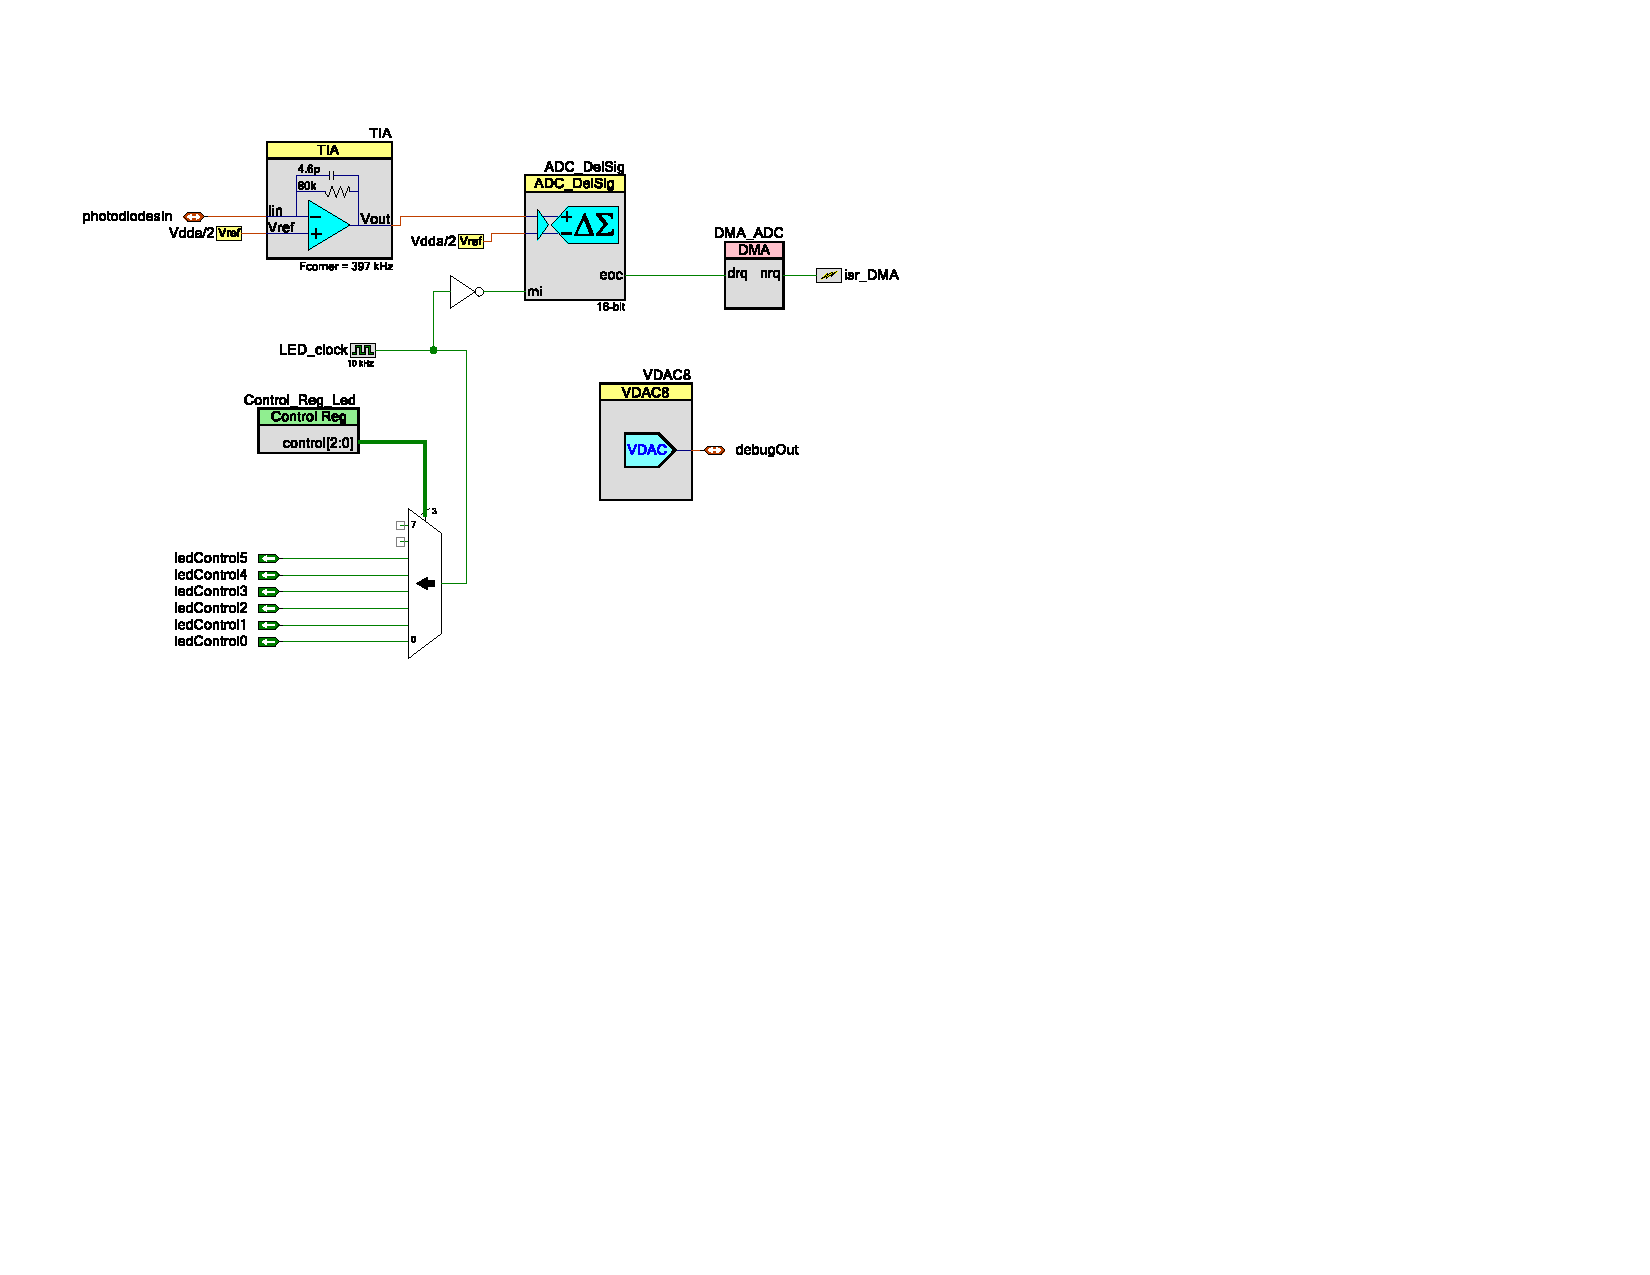
\includegraphics[width=1\columnwidth,trim={0.5in 4.1in 4.5in 0.8in},clip, page=1]{HardwareDesign/CupSensor/graphics/FinalDesign/PSoC-design.pdf}
    }
    \caption{PSoC design. 'photodiodesIn' forbindes til 'sensorsOutput' på figur \ref{fig:CupSensorCupHolderControllerPart}}
    \label{fig:CupSensorPSoCDesign}
\end{figure}

\subsubsection{Software Design}
Der er til software design af CupLight\_IF, udviklet et klassediagram, for at opnå højere samhørighed. Diagrammet kan ses på figur \ref{fig:CupSensor-IF-classDiagram}.  Klassen CupSensor\_IF er den klasse som GameController interagere med. De resterende klasser er en del af en custom component i PSoC se afsnit \ref{sec:CupSensorImplementering}. CupSensor er hoved-klassen for CupSensor blokken. CupSensor klassen har en ISR som kaldes når der kommer en ny målling fra ADC'en. 
 
\begin{figure}[H]
    \centering
    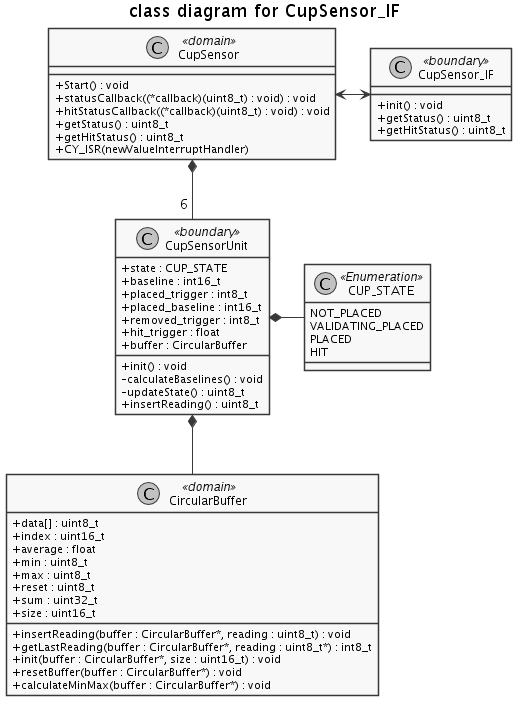
\includegraphics[width=0.8\textwidth]{Softwaredesign/CupSensor_IF/graphics/classDiagram.png}
    \caption{.}
    \label{fig:CupSensor-IF-classDiagram}
\end{figure}

Der er 6 objekter af klassen CupSensorUnit. Denne repræsentere hver Cup Sensor. Hver CupSensorUnit har en CUP\_STATE til at holde styr på tilstanden af den givne Cup Sensor. Derudover er der en CircularBuffer klasse som bruges til at lagre de seneste målinger for hver CupSensorUnit.

Der kan ses på sekvensdiagrammet på figur \ref{fig:CupSensor-IF-getting-reading} hvad der sker når der modtages en ny måling fra ADC'en. Den vigitge del i diagrammet er at når der modtages en målling fra en sensor, ændres der hvilken sensor der laves en måling på næste gang ved at styre Control\_Reg\_Led (se figur \ref{fig:CupSensorPSoCDesign}). Dette register styrer hvilken sensor der skal blinke. Derudover kaldes også insertReading metoden i den CupSensorUnit som læsningen stammer fra, bestemt af værdien af Control\_Reg\_Led. Denne metode returnerer om tilstanden ændres, hvis den gør kaldes de nødvendige metoder i GameController. 
\begin{figure}[H]
    \centering
    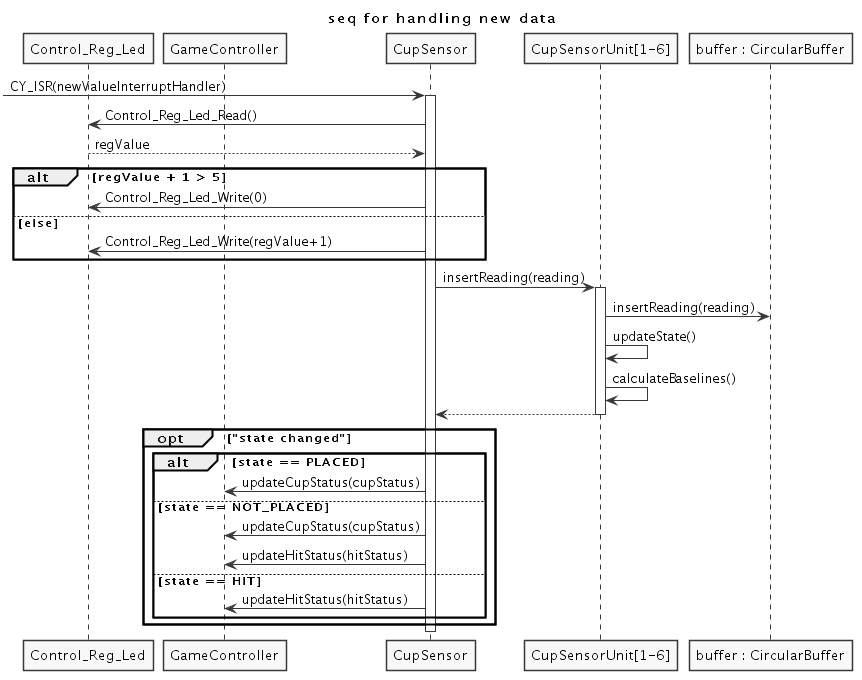
\includegraphics[width=1\textwidth]{Softwaredesign/CupSensor_IF/graphics/getting_reading.png}
    \caption{.}
    \label{fig:CupSensor-IF-getting-reading}
\end{figure}

Til at styre tilstanden for CupSensorUnit udvikles en tilstandsmaskine som ses på figur \ref{fig:CupSensor-IF-state}. 

\begin{figure}[H]
    \centering
    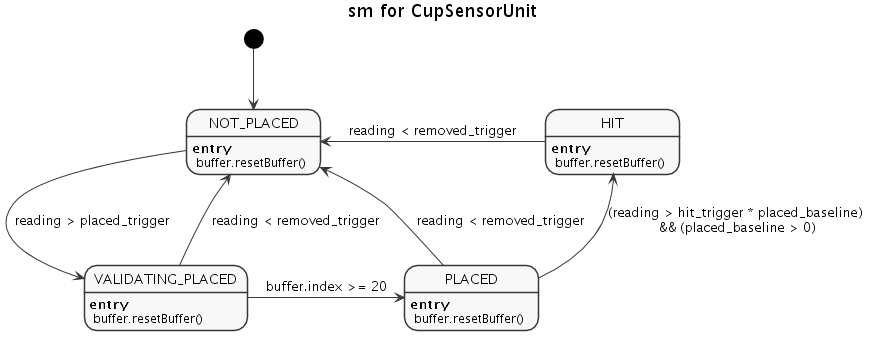
\includegraphics[width=1\textwidth]{Softwaredesign/CupSensor_IF/graphics/state.png}
    \caption{Tilstandsmaskine til CupSensorUnit.}
    \label{fig:CupSensor-IF-state}
\end{figure}

Til at bestemme de forskellige grænseværdier er der udført nogle målinger, hvor der placeres/fjernes en kop flere gange, og der tabes en bold flere gange. Dette udføres med forskellige mængder øl. Målinger og argumentation for valg af grænseværdier kan ses i \fullref{swdesign:sec:CupSensorThresholds} i Softwaredesign bilaget. 

 

\subsubsection{Implementering}\label{sec:CupSensorImplementering}
Der er valgt at lave en custom PSoC komponent kaldet CupSensor (afsnit \fullref{sec:CupSensorFinalDesign} i hardwaredesign bilag). Softwaren udvikles til PSoC vha. PSoC Creator og det er (næsten) kun muligt at benytte C. Derfor inplementeres det som 'objektorienteret C' (afsnit \fullref{swdesign:sec:CupSensorImplementation} i Softwaredesign bilaget)

\subsubsection{Modultest}
I modultesten testes sensoren ud fra de krav der er beskrevet i kravspecifikationen, samt de krav der er fra arkitekturen. De forskellige krav testes med forskellige forsyningsspændinger og mængder af øl. Den øvre, nedre og nominelle værdi, altså i alt 9 kombinationer. Der testes bl.a. antal detekteringer af placering og fjernelse af kop og antal detekteringer af bolde der rammer i koppen. (se afsnit \fullref{modultest:sec:CupSensor} i Modultest bilaget)

Resultatet af modultesten viste at der detekteres placeringer og fjernelse 100 ud af 100 gange, med 0 falske detekteringer af at en bold rammer i, for alle af de 9 kombinationer. Derudover detekteres der i den værste kombination, med $130\si{ml}$ øl og en forsyningsspænding på $5.2\si{V}$, 85 ud af 100 gange at en bold rammer i. Det måles også hvor mange falske detekteringer der kommer i forskellige scenarier. Alle disse scenarier var der 0 falske detekteringer.


\end{document}